\documentclass{beamer}
\usepackage{ragged2e}   % Package for justification
\usepackage[utf8]{inputenc}
\usepackage[english]{babel}
\usepackage[T1]{fontenc}
\usepackage{helvet}

%\useoutertheme{beaver}
%\usetheme{Warsaw}
%\usetheme{Madrid}
%\usetheme{Hannover}  % Beamer Theme

\begin{document}


\subsection{Introduction}
\begin{frame}
	\centering
	\large Unit-III\\
	\huge{Remote Procedure Calls} 
\end{frame}

\begin{frame}
	\frametitle{Introduction}
	As IPC protocol is designed for one distribute application and does not provide a 
	foundation on which to built a variety of distributed applications. Therefore, a need 
	was felt for  a general IPC protocol that can be used  for designing several 
	distributed applications. The Remote Procedure Call (RPC) facility emerged out of this 
	need.IPC gained popularity because of following reasons;
	
	\begin{enumerate}
		\item Simple Call Syntax.
		\item Familiar Semantics.
		\item Its specification of a well-defined interface.
		\item Its ease of use.
		\item Its generality.
		\item Its efficiency.
		\item It can be used as an IPC mechanism to communicate between processes on 
		different machines as well as between different processes on the same machine.
	\end{enumerate}	

\end{frame}

\subsection{RPC Model}
\begin{frame}
	\frametitle{RPC Model}
	\vspace{0.5cm}
	The RPC model is similar to the well-known and well-understood procedure call model 
	used for the transfer of control and data within a program in the following manner;
	\vspace{0.5cm}
	\begin{enumerate}
		\item To make a procedure call
		\item Control transfer
		\item Procedure body execution
		\item Returning control
	\end{enumerate}
	\vspace{0.5cm}
	\justifying{The RPC mechanism is an extension of the procedure call mechanism in the sense that it 
	enables a call to be made to a procedure that does not reside in the address space of 
	the calling process. The called procedure( commonly called remote procedure) may be on 
	the same computer or on the different computer.}\\
	\vspace{2cm}
\end{frame}

\begin{frame}
	\frametitle{RPC Model...[Contd..]}
	 Therefore the mecahnism of RPC is;
	 \begin{figure}
	 	\centering
	 	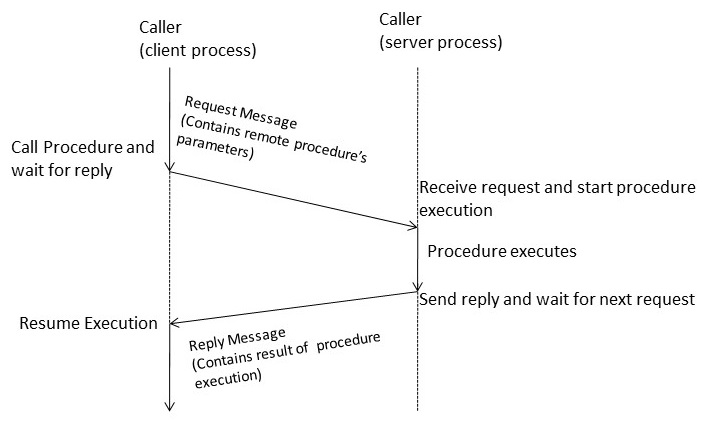
\includegraphics[width=10cm]{fig41.jpg}
	 	\caption{RPC Model}
	 \end{figure}
\end{frame}

\subsection{Transparency of RPC}
\begin{frame}
	\frametitle{Transparency of RPC}
	\justifying{A transparent RPC mechanism is one in which local procedures and remote procedures indistinguishable to the programmers. This requires the following two types of transparencies}
	\vspace{0.2cm}
	\begin{itemize}
		\item Syntactic Transparency
		\item Semantic Transparency
	\end{itemize}
	\vspace{0.5cm}
	- Syntactic transparency are easy\\
	- Semantic Transparency are not easy
	\vspace{3cm}
\end{frame}

\subsection{Implementation of RPC}
\begin{frame}
	\frametitle{Implementation of RPC}
	\justifying{Implementation of RPC mechanism usually involves the following five 
	elements of program.}
	\vspace{0.5cm}
	\begin{enumerate}
		\item Client
		\item Client Stub
		\item RPC Run time
		\item Server Stub
		\item Server
	\end{enumerate}
	\vspace{3cm}
\end{frame}

\begin{frame}
	\frametitle{Implementation of RPC...[Cntd..]}
	\begin{figure}
		\centering
		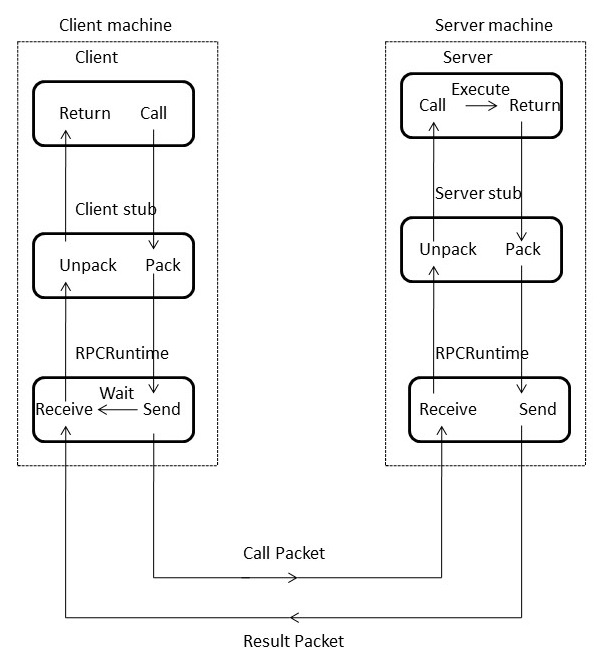
\includegraphics[width=7cm]{fig42.jpg}
		\caption{Implementation of RPC mechanism}
	\end{figure}
\end{frame}


\subsection{Stub Generation}
\begin{frame}
	\frametitle{Stub Generation}
	Stub can be generated in one of the following ways.
	\begin{itemize}
		\item Manually
		\item Automatically
	\end{itemize}
	\vspace{6cm}
\end{frame}

\subsection{RPC Messages}
\begin{frame}
	\frametitle{RPC Messages}
	There are two types of messages involved in RPC implementation.
	\begin{enumerate}
		\item Call Messages
		\item Reply Messages
	\end{enumerate}
	\vspace{1cm}
	1. Call Message\\
	\begin{figure}
		\centering
		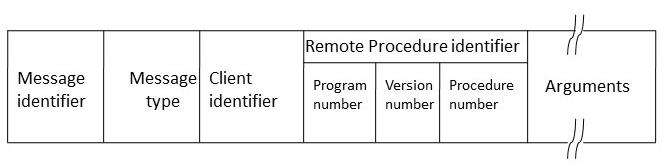
\includegraphics[width=10cm]{fig43.jpg}
		\caption{RPC Call Message Format}
	\end{figure}
\end{frame}


\begin{frame}
	\frametitle{RPC Messages...[Cntd...]}
	\vspace{0.5cm}
	2. Reply Message\\
	\begin{figure}
		\centering
		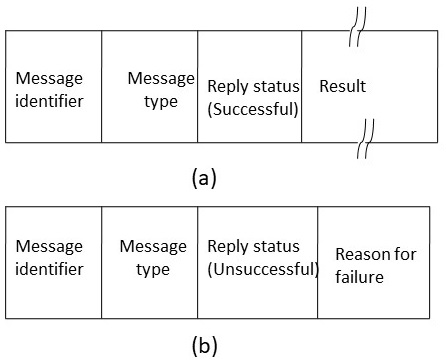
\includegraphics[width=7cm]{fig44.jpg}
		\caption{(a)A Successfule Reply Message Format (b)An Unsuccessful Message Format}
	\end{figure}
\end{frame}


\subsection{Marshaling Arguments and Results}
\begin{frame}
	\frametitle{Marshaling Arguments and Results}
	For RPC, encoding and decoding of message data is called Marshaling and involves following actions.
	\begin{enumerate}
		\item Taking the arguments
		\item Encoding the message data
		\item Decoding the message data
	\end{enumerate}
	\vspace{0.5cm}
	Marshaling procedure may be classified into two groups
	\begin{itemize}
		\item Those provided as a part of the RPC software
		\item Those that are defined by the user of the RPC system.
	\end{itemize}
	\vspace{2cm}
\end{frame}

\subsection{Server Management}
\begin{frame}
	\frametitle{Server Management}
	In IPC-based  applications, two important issues that need to be considered for server management; 
	\vspace{0.5cm}
	\begin{enumerate}
		\item Server Implementation
		\item Server Creation
	\end{enumerate}
	\vspace{5cm}
\end{frame}


\begin{frame}
	\frametitle{Server Management...[Cntd..]}
	1. Server Implementation\\
	\vspace{0.3cm}
	Based on the style of implementation used, servers may be of two types
	\vspace{0.3cm}
	\begin{itemize}
		\item Stateful Servers
		\item Stateless Servers
	\end{itemize}
		
	\vspace{5cm}
\end{frame}


\begin{frame}
	\frametitle{Server Management...[Cntd..]}
	1.1 Stateful Server
	\begin{figure}
		\centering
		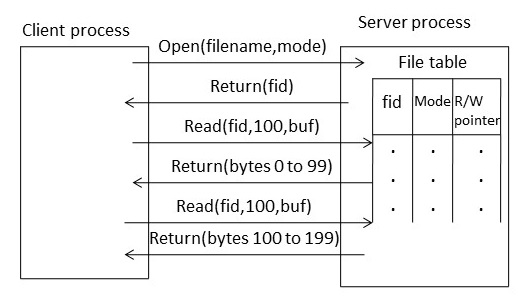
\includegraphics[width=10cm]{fig45.jpg}
		\caption{Example of a Stateful File Server}
	\end{figure}
\end{frame}

\begin{frame}
	\frametitle{Server Management...[Cntd..]}
	1.2 Stateless Servers
	\begin{figure}
		\centering
		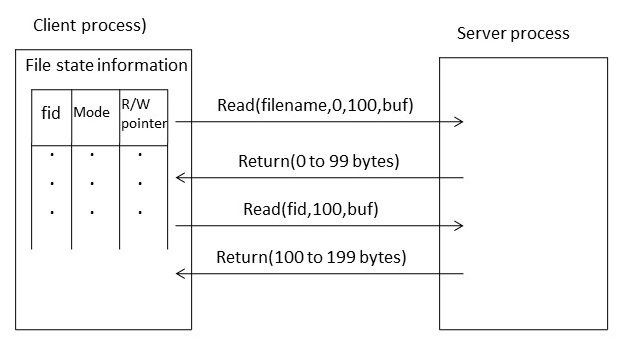
\includegraphics[width=10cm]{fig46.jpg}
		\caption{Example of a Stateless File Server}
	\end{figure}
\end{frame}

\begin{frame}
	\frametitle{Server Management...[Cntd..]}
	\vspace{0.3cm}
	2. Server Creation Semantics\\
	\vspace{0.3cm}
	Based on the time duration for which RPC server survive, they may be classified as;
	\vspace{0.3cm}
	\begin{itemize}
		\item Instance-per-Call Servers
		\item Instance-per-Session Servers
		\item Persistent Servers
	\end{itemize}
		
	\vspace{5cm}
\end{frame}

\subsection{Parameter-Passing Semantics}
\begin{frame}
	\frametitle{Parameter-Passing Semantics}
	\vspace{0.3cm}
	\justifying{The choice of parameter-Passing semantics is a crucial to the design of an 
	RPC mechanism. Followings are the choices of parameter passing;}
	\vspace{0.3cm}
	\begin{itemize}
		\item Call-by-Value
		\item Call-by-Reference
	\end{itemize}
		
	\vspace{5cm}
\end{frame}


\subsection{Call Semantics}
\begin{frame}
	\frametitle{Call Semantics}
	\vspace{0.3cm}
	\justifying{In RPC,the caller and callee processes are possibly located on different nodes. Thus it is possible for eithe the caller or callee node to fail independently and later to be restarted. In addition, failure of communication links are also possible, therefore , the normal functioning of an RPC may gets disrupted due to following reason;}
	\vspace{0.3cm}
	\begin{enumerate}
		\item The call message gets lost
		\item Response message gets lost
		\item The callee node crashes and is restarted
		\item The caller node crashes and is restarted
	\end{enumerate}		
	\vspace{5cm}
\end{frame}


\begin{frame}
	\frametitle{Call Semantics..[Cntd...]}
	\vspace{0.3cm}
	The different types of call semantics used in RPC system are;
	\vspace{0.3cm}
	\begin{enumerate}
		\item Possibly or May-be Call Semantics
		\item Last-one Call Semantics
		\item Last-of-Many Call Semantics
		\item At-Least-Once Call Semantics
		\item Exactly-Once Call Semantics
	\end{enumerate}		
	\vspace{5cm}
\end{frame}


\subsection{Communication Protocols}
\begin{frame}
	\frametitle{Communication Protocols for RPC's}
	\vspace{0.3cm}
	\justifying{Based on the needs of different systems, several communication protocols have been proposed for use of RPC's. Followings are the protocols;}
	\vspace{0.3cm}
	\begin{enumerate}
		\item The Request Protocol
		\item The Request/Reply Protocol
		\item The Request/Reply/Acknowledge-Reply Protocol
	\end{enumerate}		
	\vspace{5cm}
\end{frame}

\begin{frame}
	\frametitle{Communication Protocols for RPC's...[Cnts...]}
	\vspace{0.3cm}
	1. The Request Protocol
	\begin{figure}
		\centering
		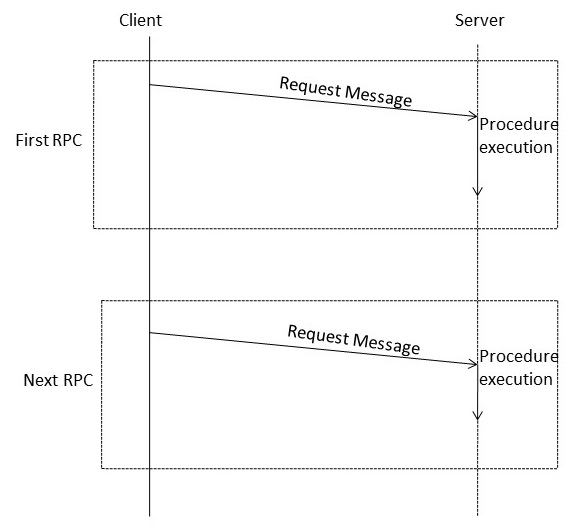
\includegraphics[width=6cm]{fig47.jpg}
		\caption{Request(R) Protocol}
	\end{figure}
\end{frame}


\begin{frame}
	\frametitle{Communication Protocols for RPC's...[Cnts...]}
	\vspace{0.3cm}
	2. The Request/Reply Protocol
	\begin{figure}
		\centering
		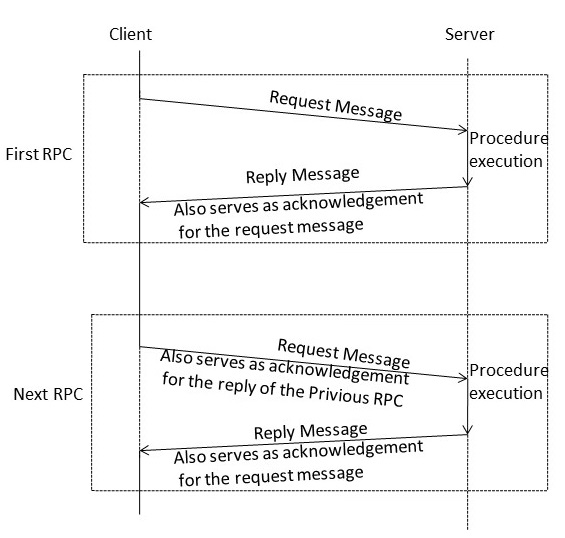
\includegraphics[width=6cm]{fig48.jpg}
		\caption{Request/Reply (RR) Protocol}
	\end{figure}
\end{frame}


\begin{frame}
	\frametitle{Communication Protocols for RPC's...[Cnts...]}
	\vspace{0.3cm}
	3. The Request/Reply/Acknowledge-Reply Protocol
	\begin{figure}
		\centering
		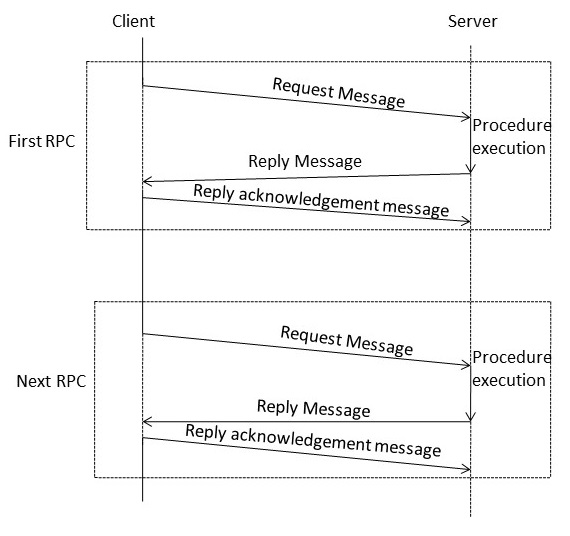
\includegraphics[width=6cm]{fig49.jpg}
		\caption{The Request/Reply/Acknowledge-Reply (RRA) Protocol}
	\end{figure}
\end{frame}


\subsection{Complicated RPCs}
\begin{frame}
	\frametitle{Complicated RPCs}
	Following two types of RPCs are complicated;
	\vspace{0.5cm}
	\begin{itemize}
		\item RPCs involving long duration calls or large gaps between calls
		\item RPCs involving arguments and /or Results that are too large to fit in a 
		single datagram packet.
	\end{itemize}
	\vspace{3cm}
\end{frame}


\subsection{Client-Server Binding}
\begin{frame}
	\frametitle{Client-Server Binding}
	The client-server binding process involves proper binding of several issues;
	\begin{enumerate}
		\item Server Naming
		\item Server Locating
		\item Binding Time
		\item Changing Binding
		\item Multiple Simultaneous Bindings
	\end{enumerate}
	\vspace{3cm}
\end{frame}

\begin{frame}
	\frametitle{Client-Server Binding...[Cntd...]}
	1. Server Naming\\
	\vspace{0.5cm}
	\begin{itemize}
		\item How does a client specify a server to which it wants to get bound?
		\item Interface Name: a type and an Instance
	\end{itemize}
	\vspace{5cm}
\end{frame}


\begin{frame}
	\frametitle{Client-Server Binding...[Cntd...]}
	2. Server Locating\\
	\vspace{0.5cm}
	To locate server, two commonly methods used
	\vspace{0.5cm}
	\begin{itemize}
		\item Broadcasting
		\item Binding Agent
		\begin{figure}
			\centering
			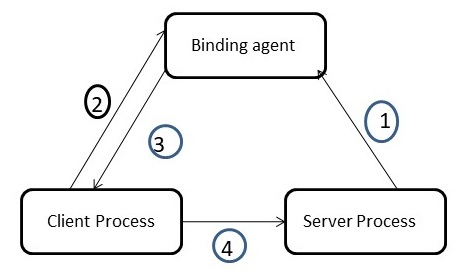
\includegraphics[width=6cm]{fig410.jpg}
			\caption{Binding Agent Mechanism for locating a server}
		\end{figure}
	\end{itemize}
\end{frame}

\begin{frame}
	\frametitle{Client-Server Binding...[Cntd...]}
	\vspace{0.5cm}
	3. Binding Time\\
	\vspace{0.5cm}
	A Client may be bound to a server at
	\vspace{0.5cm}
	\begin{itemize}
		\item Binding at Compile Time
		\item Binding at Link Time
		\item Binding at Call Time
		\begin{figure}
			\centering
			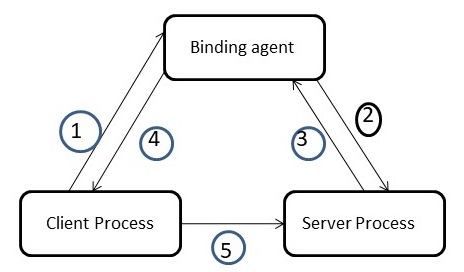
\includegraphics[width=6cm]{fig411.jpg}
			\caption{Binding at Call Time by the method of Indirect Call}
		\end{figure}
	\end{itemize}
\end{frame}


\begin{frame}
	\frametitle{Client-Server Binding...[Cntd...]}
	\vspace{0.3cm}
	4. Multiple Simultaneous Binding\\
	\vspace{0.2cm}
	In a system, a server may be provided by multiple servers. In general, a client is 
	bound to a single server of the several servers of the same time. 

	\begin{itemize}
		\item Binding at Compile Time
		\item Binding at Link Time
		\item Binding at Call Time
		\begin{figure}
			\centering
			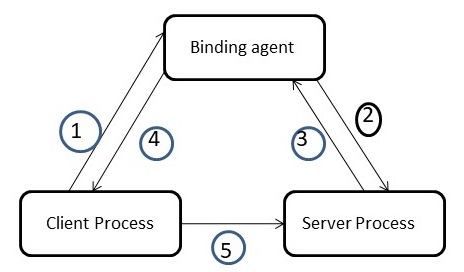
\includegraphics[width=6cm]{fig411.jpg}
			\caption{Binding at Call Time by the method of Indirect Call}
		\end{figure}
	\end{itemize}
\end{frame}


\begin{frame}
	\frametitle{Some Special Types of RPC's}
	\vspace{0.2cm}
	1. Callback RPC
	\begin{figure}
		\centering
		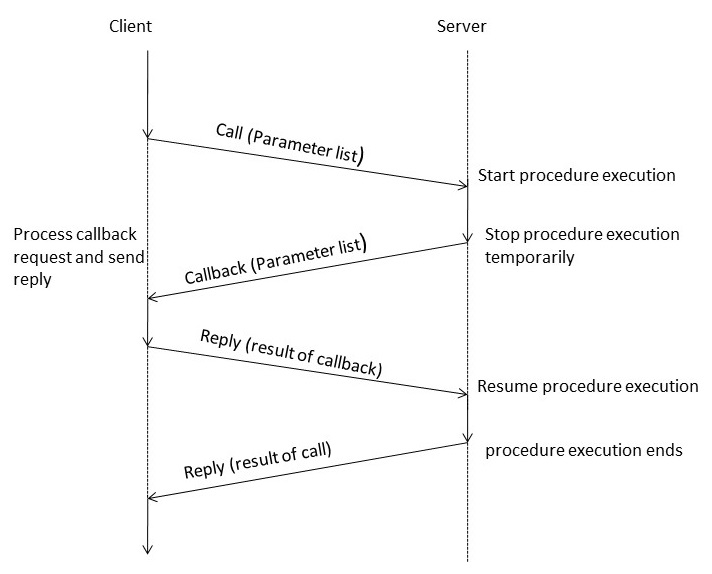
\includegraphics[width=8.5cm]{fig412.jpg}
		\caption{Callback RPC}
	\end{figure}
\end{frame}

\begin{frame}
	\frametitle{Some Special Types of RPC's...[Cntd...]}
	\vspace{0.5cm}
	To provide callback RPC facilities, followings are necessary
	\vspace{0.5cm}
	\begin{itemize}
		\item Providing the Server with the Client's Handle
		\item Making the Client Process Wait for the Callback RPC
		\item Handling Callback Deadlocks
		\begin{figure}
			\centering
			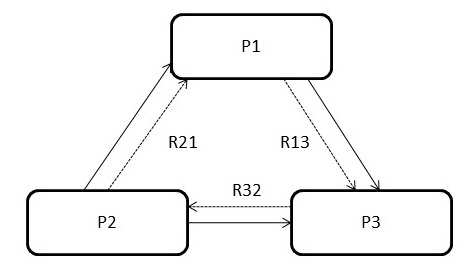
\includegraphics[width=7cm]{fig413.jpg}
			\caption{Callback Deadlock}
		\end{figure}
	\end{itemize}
\end{frame}


\begin{frame}
	\frametitle{Some Special Types of RPC's...[Cntd...]}
	2. Broadcast RPC\\
	\vspace{0.5cm}	
	A broadcast RPC mechanism may use one of the following two methods for broadcasting a 
	clients request;
	\begin{itemize}
		\item A special broadcast primitives
		\item To declare broadcast ports
	\end{itemize}	
	\vspace{4cm}	
\end{frame}


\begin{frame}
	\frametitle{Some Special Types of RPC's...[Cntd...]}
	\vspace{0.5cm}
	3. Batch-Mode RPC\\
	\vspace{0.5cm}
	\begin{itemize}
		\item{mode RPC is used to queue separate RPC request in a transmission 
		buffer on the client side and then send them over the network in one batch to the 
		server.}\\
		\vspace{0.5cm}
		\item{However, batch-mode RPC can be used only with those applications in which a 
		client has many RPC requests to send to a server and the client does not need to 
		reply for a sequence of requests.}\\
		\vspace{0.5cm}
		\item{Therefore, the requests are queued on the client side and the entire queue 
		of 	requests is flushed to the server.}

	\end{itemize}
		\vspace{1.8cm}
\end{frame}


\subsection{RPC in Heterogeneous Environment}
\begin{frame}
	\frametitle{RPC in Heterogeneous Environment}
	\justifying{When designing an RPC system for a heterogeneous environment, the three 
	common types of heterogeneity that need to be considered}
	\vspace{0.5cm}
	\begin{enumerate}
		\item Data Representation
		\item Transport Protocol
		\item Control Protocol
	\end{enumerate}
	\vspace{3cm}
\end{frame}


\subsection{Lightweight RPC}
\begin{frame}
	\frametitle{Lightweight RPC}
	\justifying{To achieve better performance than conventional RPC, following four 
	techniques are used by LRPC}
	\begin{enumerate}
		\item Simple Control Transfer
		\item Simple Data Transfer
		\item Simple Stubs
		\item Design for Concurrency
	\end{enumerate}
	\vspace{4cm}
\end{frame}


\begin{frame}
	\frametitle{Lightweight RPC...[Cntd...]}
	\begin{figure}
		\centering
		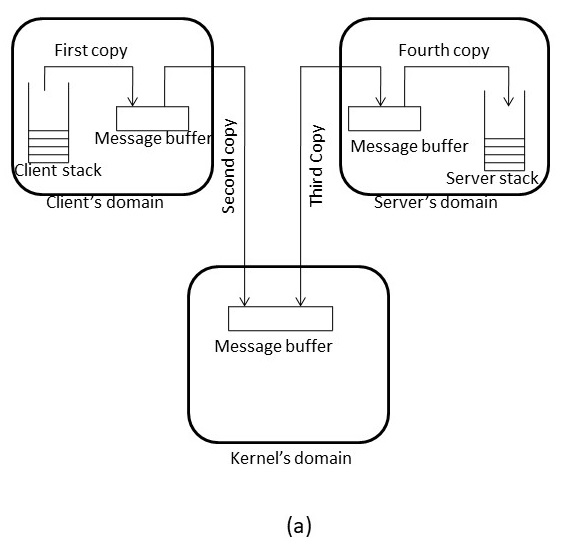
\includegraphics[width=7cm]{fig414(a).jpg}
		\caption{(a)Tradittional Cross Domain RPC}
	\end{figure}				
\end{frame}


\begin{frame}
	\frametitle{Lightweight RPC...[Cntd...]}
	\begin{figure}
		\centering
		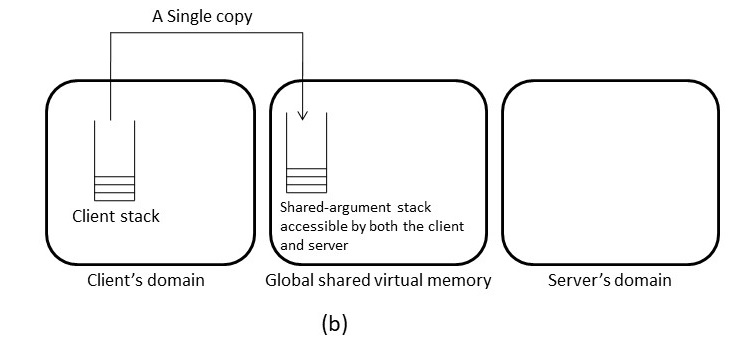
\includegraphics[width=10cm]{fig414(b).jpg}
		\caption{(b)LightWeight RPC}
	\end{figure}
\end{frame}





\end{document}